\documentclass[11pt,a4paper,oneside]{article}
\usepackage[latin1]{inputenc}
\usepackage{amsmath}
\usepackage{amsfonts}
\usepackage{amssymb}
\usepackage{graphicx}
\usepackage{color}
\usepackage {tikz}
\usepackage{fancyvrb}
\usetikzlibrary {er}
\usepackage[left=2.00cm, right=2.00cm, top=1.00cm]{geometry}
\graphicspath{{./}}
\fvset{tabsize=4}

\begin{document}
	\title{DS 255 - System Virtualization \\ Assignment I - OS Primer}
	\author{Shriram R. \\ M Tech (CDS) \\ 06-02-01-10-51-18-1-15763}
	\maketitle	
	
	\begin{enumerate}
		\item Modern ISAs like Intel x86 support four different execution privileges or protection rings with one for OS Kernel, two for OS Services and one for the Applications. OS Kernel has the highest privilege while the Application will have the lowest privilege. This is illustrated in the figure given below,
		      \begin{center}
		         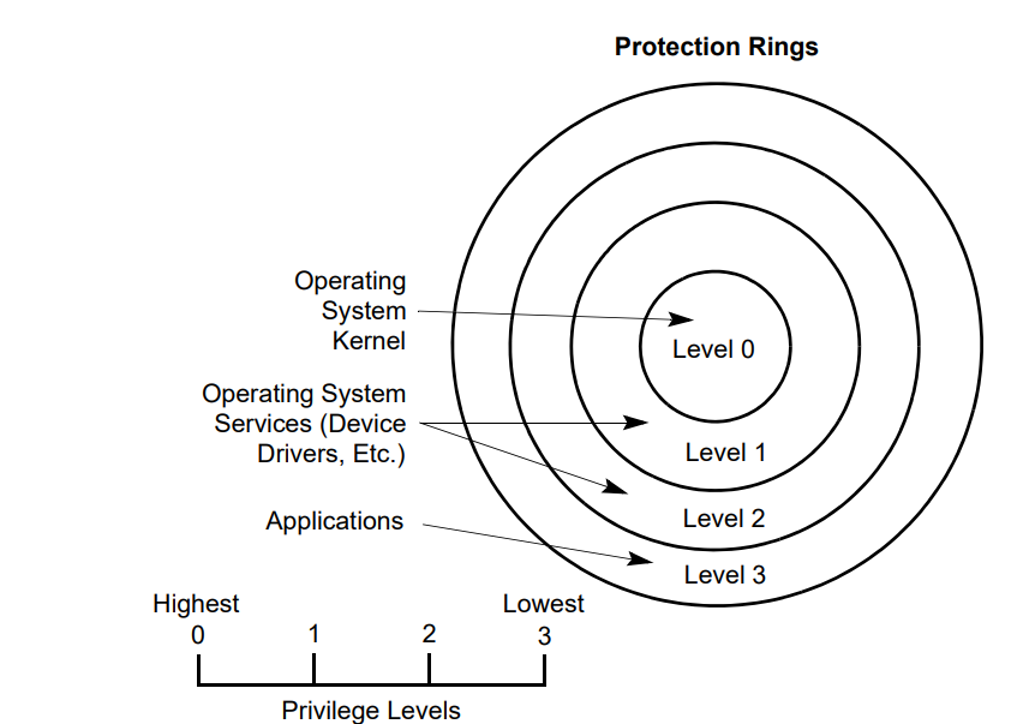
\includegraphics[scale=0.4]{1.png}	
		         [1]	
		      \end{center}
		These privileges are necessary to enable the OS to establish control over the system and restrict user processes from gaining arbitrary access to more resources or memory space of other processes. Modern Operating systems typically support Level 0 (Kernel) and Level 3 (User) execution modes.
		
		For x86, the current mode of execution can be determined by examining the lower two bits set in code segment register. This should be similar in the other architectures as well.
		
		A proess can change its privilege from user mode to kernel mode by making a system call. Note that a process cannot execute arbitrary instructions of its own during kernel mode. The following happens when a system call is made,
		\begin{enumerate}
			\item Process registers are saved to kernel stack and mode is changed to kernel mode
			\item OS trap handler performs execution of its code in kernel mode
			\item After trap handler completes execution, process registers are restored from the process stack and mode is changed to user mode
			\item Process continues execution in user mode   
		\end{enumerate} 
	   
	    \begin{verbatim}
	    
	    
	    
	    
	    \end{verbatim}
	
		
		\item The schematic of process address space organization in 32-bit Linux is given below,
				  \begin{center}
				  	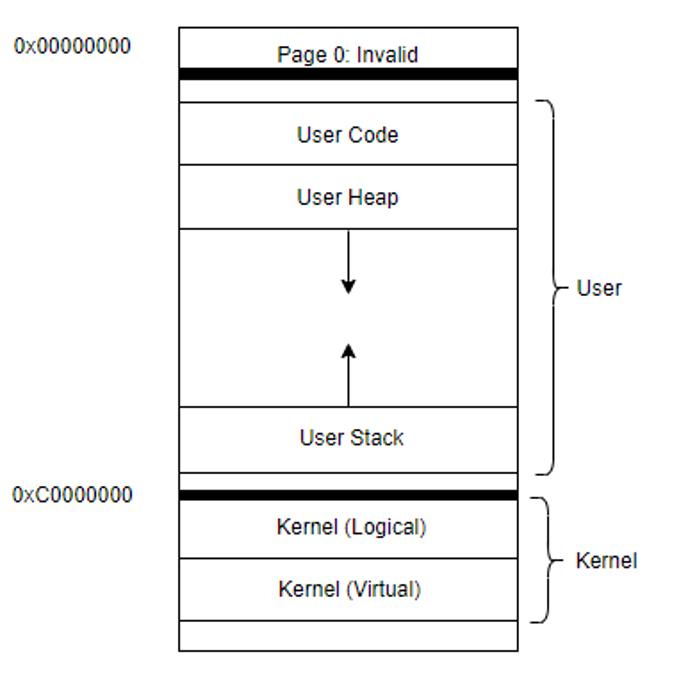
\includegraphics[scale=0.5]{2.png}	[2]	
				  \end{center}
		The split between user (process) and kernel space is present at 0xC0000000 which is 75\% through the space. The heap and stack space of a process can grow and shrink dynamically. Note that the heap space grows in the increasing address direction while the stack space grows in the decreasing direction. 
		
		The kernel logical address space holds most of the kernel data structures. There exists a direct mapping between kernel logical address and the first part of physical memory. This implies that the kernel logical memory is contiguous in the physical memory as well.
		
		The kernel virtual address is not physically contiguous and these are typically used for allocating large buffers. Note that a process will not have access to the entire kernel memory space.
		
		\item A process interfaces to I/O devices in UNIX like systems through files (file descriptors). Concurrency has to be handled by the interface (i.e) the requests made to I/O device has to be serialized by the interface provided by OS. 
		
		Unix based systems provide \emph{flock()} system call which can be used to apply or remove an advisory lock on an open file. For example, if cooperating two processes A and B are writing concurrently to a file F, the processes can coordinate by using an exclusive lock on F. The process (A or B) which acquires the lock will write to the file while the other process will get blocked waiting for the lock. A pseudocode for the operation is given below,
		
		\begin{verbatim}
		   // Pseudocode for process A and B
		   flock(fd, LOCK_EX); // Blocked till lock is acquired
		   // Do any write operation on fd
		   write(fd, *buf, count);
		   flock(fd, LOCK_UN); // Unlock
		\end{verbatim} 
		
		It must be noted that the locks are advisory. This means that if two non-cooperating process which are not using locks are trying to write concurrently to a file, they can end up doing so and overwrite each other's data.
		
		 \begin{verbatim}


		\end{verbatim}
			
		\item The control flow diagram to read a record from a file in disk is given below,
		
		     \begin{center}
		     	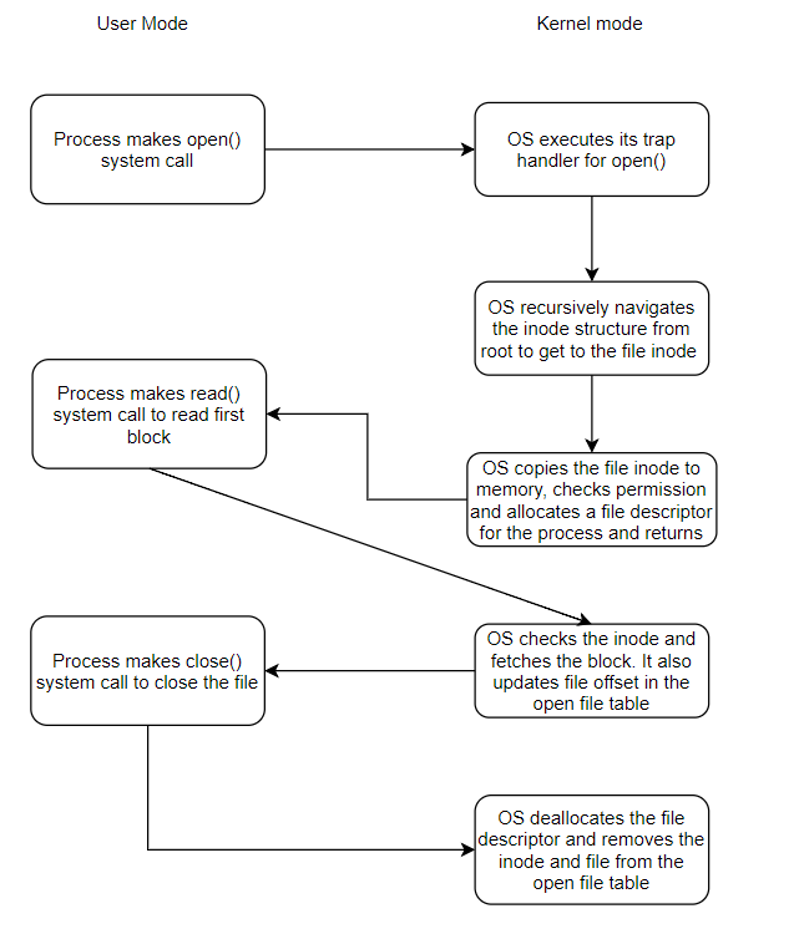
\includegraphics[scale=0.7]{3.png}
		     \end{center}
		
		Filesystem cache buffer is used to hold popular disk blocks in memory to improve performance. The buffer size can be static or dynamic and policies like LRU is used to decide which blocks to be replaced in the buffer. 
		
		This buffer can greatly improve performance of read and writes. In the case of writes, multiple write operations can be batched together and the OS can efficiently schedule the actual I/O operations. However, applications like databases would have issues in buffering as they would want to flush all writes to disk when needed. For this purpose, OS provides fsync() call to flush any dirty blocks in a file to the disk.
		
		 			
				
	\end{enumerate}
    
    \textbf{References}
    \begin{enumerate}
    	\item Intel\textsuperscript{�} 64 and IA-32 Architectures Software Developer's Manual Combined Volumes: 1, 2A, 2B, 2C, 2D, 3A, 3B, 3C, 3D, and 4
    	\item Operating Systems: Three Easy Pieces, Remzi H. Arpaci-Dusseau and Andrea C. Arpaci-Dusseau, Arpaci-Dusseau Books.
    \end{enumerate}
 

    
\end{document}